\documentclass[twocolumn,showpacs,floatfix,nofootinbib,longbibliography]{revtex4-1}
\usepackage{graphicx}
\usepackage{bm} % bold math
\usepackage{amssymb} % use this package to enable \nrightarrow command
\usepackage{amsmath} % use this package to enable \xrightarrow command
\usepackage{braket} % use for Dirac bra-kets : \rangle \labgle & \mid
\usepackage{natbib} % bibtex package
\usepackage{hyperref}


\begin{document}

\title{Currents induced by magnetic impurities in superconductors with spin-orbit coupling}

\author{Sho Nakosai$^{1,2}$}
\author{Sergey S. Pershoguba$^{2}$}
\author{Alexander V. Balatsky$^{,3}$}
\affiliation{$^1$Department of Applied Physics, University of Tokyo, Tokyo 113-8656, Japan}
\affiliation{$^2$Nordita, Center for Quantum Materials, KTH Royal Institute of Technology, and Stockholm University, Roslagstullsbacken 23, S-106 91 Stockholm, Sweden}
\affiliation{$^3$Institute for Materials Science, Los Alamos National Laboratory, Los Alamos, NM 87545, USA}

\date{\today}


\begin{abstract}
Skyrmions are nice
\end{abstract}

\pacs{ }   

%%%%%%%%%%%%%%%%%%%%%%%%%%%%%%%%%%%%%%%%%%%%%%%%%%%%%%%%%%%%%%%%%%%%%%%%%%

\maketitle
%%%%%%%%%%%%%%%%%%%%%%%%%%%%%%%%%%%%%%%%%%%%%%%%%%%%%%%%%%%%%%%%%%%%%%%%%%%
\section{Introduction} \label{sec:intro}
%%%%%%%%%%%%%%%%%%%%%%%%%%%%%%%%%%%%%%%%%%%%%%%%%%%%%%%%%%%%%%%%%%%%%%%%%%%

General context of skyrmions asd tolopolical excitations: memory, manipulation, local creation via SP STM.
Extension of skyrmion discussion to the case of hybrid structures: SC and Skyrmion. What are the consequenc of brining topological exchange field into SC. Question we address is the possible local spectroscopic signatures of SC quasiparticles in SC due to skyrmion field. We know from the past discussion that there are impurity bound states in SC near magnetic impurities. We have now the framework to address formation of bound states. Talk about local single impurity limit (YSR) and show the cartoon of the local and extended skyrmion and spectra. There are two effects: local scattering and Zeeman field hence the DOS will be split etc.  Draw similarities and differences with single imp.
In parallel with skyrmion discovery the local imaging using magnetic probes like MFM and SP-STM allowed one to image the matter at atomic resolution while also resolving spin content of electron carriers in the substrate.  
Here we prove the existence of the new type of localized excitation on the skyrmion core we call  Sc-YSR state (alternative is skyrmion bound state (sbs)).  Show the main results upfront in the introduction. Both LDOS and SP-LDOS. 
Main section: 

Introduce T matrix and results for analytic solution.  
Introduce the numerical approach and presenst the results oas a function of position and as a function of energy. Kind of same figs as in Sho’s talk. 
Discuss the results and what it means, how big the signal is etc. Unfortunately we do not see any topological state at zero energy and as such these result represent a new kind of magnetic texture induced states that exhibit intragap states.


%%%%%%%%%%%%%%%%%%%%%%%%%%%%%%%%%%%%%%%%%%%%%%%%%%%%%%%%%%%%%%%%%%%%%%%%%%%
\section{Skyrmions in ferromagnetic films} \label{sec:skyrmion}
%%%%%%%%%%%%%%%%%%%%%%%%%%%%%%%%%%%%%%%%%%%%%%%%%%%%%%%%%%%%%%%%%%%%%%%%%%

%%%%%%%%%%%%%%%%%%%%%%%%%%%%%%%%%%%%%%%%%%%%%%%%%%%%%%%%%%%%%%%%%%%%%%%%%%%
\begin{figure} \centering
(a) 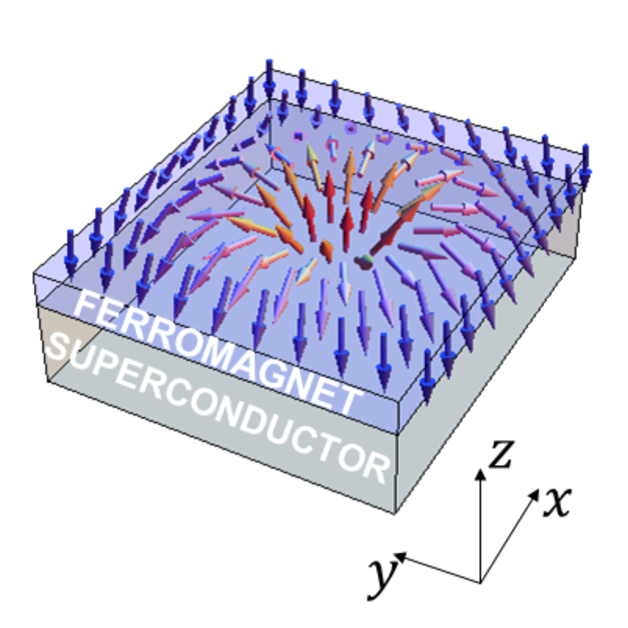
\includegraphics[width=0.4\linewidth]{SkyrmA}  
(b) 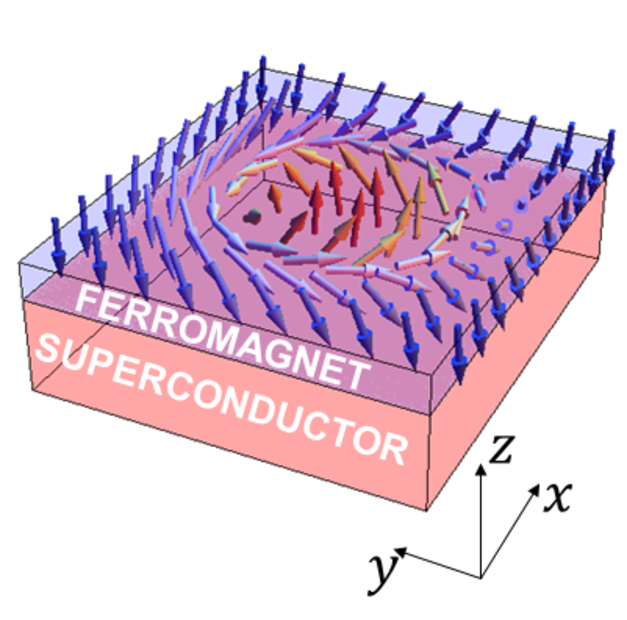
\includegraphics[width=0.4\linewidth]{SkyrmB} 
\caption{(Color online.) Ferromagnetic field with skyrmion configuration of magnetism on top of a superconductor. (a) Monopole skyrmion.  (b) Anapole skyrmion. } \label{fig:skyrmion}
\end{figure}
%%%%%%%%%%%%%%%%%%%%%%%%%%%%%%%%%%%%%%%%%%%%%%%%%%%%%%%%%%%%%%%%%%%%%%%%%%




Let the three-dimensional vector $S(\bm r) = (S_x,S_y,S_z)$ describe the configuration of the ferromagnetic vector in a two-dimensional ferromagnetic film $\bm r = (x,y)$. The configurations of the field $S(\bm r)$ shown in Fig. \ref{fig:skyrmion}(a) and (b) are referred to as skyrmions. The skyrmion configuration of the field is characterized by the topological charge 

\begin{align}
	Q = \frac{1}{4\pi} \int d^2r \, \hat {\bm S}\cdot (\nabla_x\hat {\bm S}\times\nabla_y\hat {\bm S}), \quad \hat {\bm S}= \frac{\bm S}{S}, 
	\label{topCharge}
\end{align}
which cannot be altered by the continuous transfomation of the field.  We also characterize the skyrmion fields by the zeroth and first moments
\begin{align}
	S^{(0)}_i = \int  d^2r \, \left[S_i(\bm r)-S_i(\infty)\right], \\
	S^{(1)}_{ij} = \int  d^2r \, \left[S_i(\bm r)-S_i(\infty)\right] r_j.
	\label{moments}
\end{align}
The zeroth moment defines the average moment of the skyrmion and it is equal for the two skyrmions shown in Fig.~{\ref{fig:skyrmion}}(a) and (b). For the cylindrically symmetric field $S(\bm r)$, the first order moment can be expanded in the symmetric and antisymmetric parts $S^{(1)}_{ij}=S^{(1)}_{\rm monopole}\,\delta_{ij} + S^{(1)}_{\rm anapole}\,\epsilon_{ijz}$. The skyrmions shown in Fig.~\ref{fig:skyrmion}(a) and (b) have monopole and anapole moments correspondingly, hence the name of the skyrmions. However the two types of the skyrmions have the same topological charge~(\ref{topCharge}) and thus can be continuosly deformed into each other. 



%%%%%%%%%%%%%%%%%%%%%%%%%%%%%%%%%%%%%%%%%%%%%%%%%%%%%%%%%%%%%%%%%%%%%%%%%%%
\section{T-matrix analysis} \label{sec:analytics}
%%%%%%%%%%%%%%%%%%%%%%%%%%%%%%%%%%%%%%%%%%%%%%%%%%%%%%%%%%%%%%%%%%%%%%%%%%%
Superconductor-ferromagnet heterostructures were recently proposed as a viable platform for realizing topological superconductivity (TS) \cite{Lutchyn2010,Oreg2010, Sau2010}, which can host Majorana fermion quasiparticles at vortex cores and boundaries \cite{Kitaev2001, Alicea, Beenakker2013}. Majorana fermions obey non-Abelian statistics and may be utilized for topological quantum computation \cite{Read2000, Ivanov2001, Nayak2008}.  The key ingredients driving these systems in the topologically non-trivial regime are the spin-orbit coupling (SOC) and magnetism. Recently, the search for experimental realizations of TS has also led to engineering the impurity bands of the Yu-Shiba-Rusinov (YSR) states \cite{Yu,Shiba,Rusinov}, induced by magnetic atoms on the surface of a superconductor \cite{Choy2011, Nadj-Perge2013, Klinovaja2013, Vazifeh2013, Braunecker2013, Pientka2013, Nakosai2013, Poyhonen2014, Reis2014, Brydon2015, Rontynen2014, Li2015}. Following this recipe, zero-energy peaks in the tunneling spectrum were recently measured at the ends of a one-dimensional (1D) chain of magnetic atoms \cite{Yazdani2014}. Such a tunneling spectrum could be the evidence of Majorana edge states, although alternative explanations are also possible \cite{Sau2015}.




\begin{equation}
 T = \frac{V}{1-vg_{00}}
\end{equation}

%%%%%%%%%%%%%%%%%%%%%%%%%%%%%%%%%%%%%%%%%%%%%%%%%%%%%%%%%%%%%%%%%%%%%%%%%%%
\section{Numerical analysis} \label{sec:numerics}
%%%%%%%%%%%%%%%%%%%%%%%%%%%%%%%%%%%%%%%%%%%%%%%%%%%%%%%%%%%%%%%%%%%%%%%%%%%
Text added by Sho.
2nd edition. 
Another addition. 
Further addition.
No more addition.
%%%%%%%%%%%%%%%%%%%%%%%%%%%%%%%%%%%%%%%%%%%%%%%%%%%%%%%%%%%%%%%%%%%%%%%%%%%
\section{Conclusion} \label{sec:conclusion}
%%%%%%%%%%%%%%%%%%%%%%%%%%%%%%%%%%%%%%%%%%%%%%%%%%%%%%%%%%%%%%%%%%%%%%%%%%%




\newpage
%%%%%%%%%%%%%%%%%%%%%%%%%%%%%%%%%%%%%%%%%%%%%%%%%%%%%%%%%%%%%%%%%%%%%%%%%%%%%
%\bibliographystyle{apsrev4-1}
\bibliography{Skyrmion}
%%%%%%%%%%%%%%%%%%%%%%%%%%%%%%%%%%%%%%%%%%%%%%%%%%%%%%%%%%%%%%%%%%%%%%%%%%%%%


\end{document}
